%-----------------------------------------------------------------------------%
\chapter{\babTiga}
\label{bab:3}
%-----------------------------------------------------------------------------%
Bab ini menjelaskan proses perancangan dari aplikasi yang dikembangkan penulis. Proses perancangan dimulai dari menjelaskan metode penelitian, analisis kebutuhan, identifikasi fitur, dan perancangan arsitektur aplikasi.


\section{Metode Penelitian}
\label{sec:metodePenelitian}

Gambar \ref{fig:alur-penelitian} menjelaskan alur umum dari penelitian yang akan dilakukan penulis. Berikut adalah penjelasan singkat mengenai setiap fase pada ilustrasi tersebut:

\begin{enumerate}
    \item \textbf{Studi Literatur}: Melakukan studi literatur awal mengenai helm dan penggunaan helm dan mengenai implementasi Helm API yang serupa. Penulis juga akan melakukan studi literatur mengenai integrasi Vault, Amazon Kinesis, dan Templating.
    \item \textbf{Analisis Kebutuhan}: Mengumpulkan kebutuhan dari pengguna. Kebutuhan didapatkan dari wawancara yang dilakukan oleh penulis kepada pengguna saat masa perancangan aplikasi.
    \item \textbf{Identifikasi Fitur}: Dari kebutuhan yang telah dikumpulkan selama masa analisis kebutuhan, akan dikumpulkan fitur yang akan dimiliki oleh aplikasi.
    \item \textbf{Perancangan Fungsi Aplikasi}: Akan dibuat daftar fungsi-fungsi yang dapat digunakan pada aplikasi.
    \item \textbf{Perancangan Arsitektur Lingkungan Kubernetes}: Penulis akan merancang skema arsitektur Kubernetes dimana aplikasi yang dikembangkan akan berjalan.
    \item \textbf{Perancangan Arsitektur Aplikasi}: Penulis akan merancang skema arsitektur aplikasi berdasarkan kebutuhan fitur yang telah dikumpulkan.
    \item \textbf{Implementasi Program}: Akan dilakukan implementasi aplikasi berdasarkan rancangan yang telah disusun pada tahapan analisis dan perancangan.
    \item \textbf{Implementasi Kebutuhan \textit{Deployment}}: Mengkonfigurasikan kebutuhan-kebutuhan yang diperlukan agar aplikasi yang telah dikembangkan dapat berjalan pada \textit{server}.
    \item \textbf{Proses \textit{Deployment}}: Penulis melakukan proses \textit{deployment} aplikasi kedalam lingkungan kerja milik PT Gudang Ada Globalindo.
    \item \textbf{Pengujian}: Penulis akan melakukan pengujian aplikasi dari kebutuhan yang telah dispesifikasikan.
\end{enumerate}

\begin{figure}
	\centering
	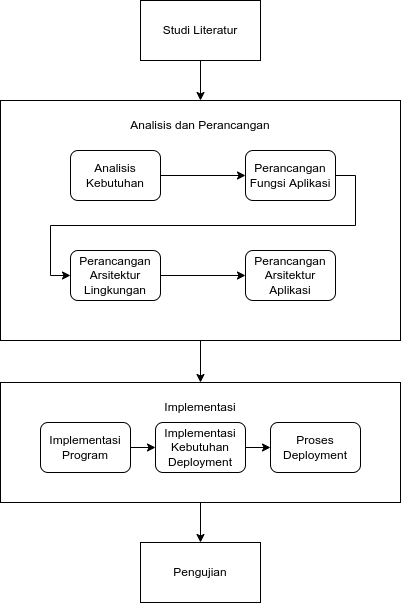
\includegraphics[width=0.8\textwidth]{pics/MetodePenelitian.png}
	\caption{Alur penelitian penulis}
	\label{fig:alur-penelitian}
\end{figure}

%-----------------------------------------------------------------------------%
\section{Analisis Kebutuhan}
\label{sec:analisisKebutuhan}
%-----------------------------------------------------------------------------%
Dikumpulkan kebutuhan melalui diskusi dengan \textit{user} yang dilakukan selama masa penelitian. Dari hasil diskusi tersebut, didapatkan kebutuhan pengguna dapat dilihat dari tabel berikut:

\begin{table}
    \centering
    \begin{tabular}{|c|p{12cm}|}
        \hline
        \multicolumn{1}{|c|}{Kode} & \multicolumn{1}{c|}{\textbf{Kebutuhan Pengguna (K)}} \\
        \hline
        K1 & Pengguna dapat melakukan \textit{deployment} satu atau lebih helm sekaligus. \\
        \hline
        K2 & Pengguna dapat melakukan \textit{deployment} pada \textit{namespace} Kubernetes yang berbeda-beda \\
        \hline
        K3 & Pengguna dapat membuat satu atau lebih Amazon Kinesis \textit{instance} sekaligus. \\
        \hline
        K4 & Pengguna akan melakukan banyak \textit{deployment} dengan spesifikasi yang mirip. \\
        \hline
        K5 & \textit{Repository} Helm Chart yang sedang dipakai harus tetap dipakai. \\
        \hline
        K6 & Pengguna dapat melakukan perubahan pada \textit{service} yang sudah di \textit{deploy}. \\
        \hline
        K7 & Pengguna dapat menghapus \textit{service} yang sudah di \textit{deploy}. \\
        \hline
        K8 & \textit{Service} yang dapat dihapus hanyalah \textit{service} yang di \textit{deploy} oleh aplikasi, bukan \textit{service} lain yang berada pada lingkungan yang sama \\
        \hline
        K9 & Pengguna dapat melihat detail dari \textit{service} yang sudah di \textit{deploy}. \\
        \hline
        K10 & Pengguna dapat melakukan \textit{deployment} aplikasi yang memiliki \textit{secret environment variable} tanpa mengetahui variabel tersebut. \\
        \hline
    \end{tabular}
    \caption{Identifikasi Kebutuhan}
    \label{tab:analisisKebutuhanPengguna}
\end{table}

\section{Identifikasi fitur}
\label{sec:identifikasiFitur}

Data dari tabel \ref{tab:analisisKebutuhanPengguna} dapat ditranformasikan menjadi spesifikasi yang diinginkan pada aplikasi yang akan dikembangkan. Hasil dari analisis tersebut akan dijadikan kebutuhan teknis yang dapat dilihat pada tabel \ref{tab:analisisFitur}:
\begin{table}
    \centering
    \begin{tabular}{|c|p{11cm}|p{1.5cm}|}
        \hline
         &  & \multicolumn{1}{|c|}{\textbf{Kode}} \\
        \multicolumn{1}{|c|}{\textbf{Kode}} &  \multicolumn{1}{c|}{\textbf{Kebutuhan Fitur Aplikasi (F)}} & \multicolumn{1}{|c|}{\textbf{Referensi}}\\
        & & \multicolumn{1}{|c|}{\textbf{K}} \\
        \hline
        F1 & Aplikasi memiliki fitur \textit{templating} yang dapat mengintegrasikan banyak \textit{deployment} sekaligus. & K1, K3, K4\\
        \hline
        F2 & Aplikasi dapat melayani proses \textit{deployment} Helm. & K1, K2\\
        \hline
        F3 & Aplikasi dapat melayani proses \textit{deployment} Amazon Kinesis. & K3\\
        \hline
        F4 & Aplikasi berintegrasi dengan Amazon S3 sebagai tempat penyimpanan Helm Chart. & K5\\
        \hline
        F5 & Terdapat \textit{persistence layer} yang dapat mencatat \textit{deployment}, perubahan \textit{deployment}, dan penghapusan \textit{deployment}. & K6, K7, K8, K9\\
        \hline        
    \end{tabular}
    \caption{Identifikasi Fitur}
    \label{tab:analisisFitur}
\end{table}
%-----------------------------------------------------------------------------%

\section{Perancangan Fungsi Aplikasi}
\label{sec:penggunaanAplikasi}

Aplikasi yang akan dikembangkan memiliki beberapa fitur yang telah dikumpulkan pada tabel \ref{tab:analisisFitur}. Fitur tersebut akan di akses oleh pengguna melalui beberapa fungsi. Bagian ini akan menjelaskan fungsi-fungsi yang dapat dipanggil oleh pengguna yang disediakan oleh aplikasi.

\subsection{Helm}
\label{sec:helmFeature}

Aplikasi yang dikembangkan harus dapat melakukan proses \textit{deployment} Helm. Adapun fungsi yang disediakan oleh aplikasi adalah sebagai berikut:

\begin{itemize}
    \item Membuat \textit{deployment} Helm.
    \item Melihat seluruh \textit{deployment} Helm.
    \item Melihat detail dari suatu \textit{deployment} Helm.
    \item Mengubah data dari suatu \textit{deployment} Helm.
    \item Menghapus suatu \textit{deployment} Helm.
\end{itemize}

\subsection{Kinesis}

Aplikasi yang dikembangkan harus dapat membuat \textit{instance} Amazon Kinesis. Adapun fungsi yang disediakan oleh aplikasi adalah sebagai berikut:

\begin{itemize}
    \item Membuat \textit{instance} Amazon Kinesis.
    \item Melihat seluruh \textit{instance} Amazon Kinesis.
    \item Melihat detail dari suatu \textit{instance} Amazon Kinesis.
    \item Mengubah data dari suatu \textit{instance} Amazon Kinesis.
    \item Menghapus suatu \textit{instance} Amazon Kinesis.
\end{itemize}

\subsection{Templating}

Aplikasi yang dikembangkan juga harus dapat membuat sistem \textit{templating} yang dapat melakukan \textit{deployment} Helm dan pembuatan \textit{instance} Amazon Kinesis. Aplikasi tersebut juga harus dapat mengakses variabel rahasia agar dapat mengamankan proses \textit{deployment}. Adapun fungsi yang disediakan oleh aplikasi adalah sebagai berikut:

\begin{itemize}
    \item Membuat definisi \textit{template deployment}.
    \item Melakukan \textit{deployment} berdasarkan \textit{template} yang telah didefinisikan.
    \item Melihat semua \textit{deployment}.
    \item Melihat detail dari sebuah \textit{deployment}.
    \item Mengubah \textit{deployment}.
    \item Menghapus \textit{deployment}.
\end{itemize}

\section{Perancangan Arsitektur Lingkungan Kubernetes}
\label{sec:perancanganEnvironment}
Aplikasi yang dikembangkan perlu di \textit{deploy} dan dikonfigurasikan sesuai kebutuhan pengguna. Aplikasi yang telah dikembangkan akan dikemas keladalam kontainer seperti gambar \ref{fig:aplikasiDiDalamKontainer}. 

\begin{figure}
	\centering
	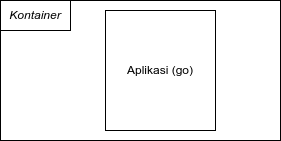
\includegraphics[width=0.5\textwidth]{pics/AplikasiDalamKontainer.png}
	\caption{Aplikasi di dalam kontainer}
	\label{fig:aplikasiDiDalamKontainer}
\end{figure}

Kontainer pada gambar \ref{fig:aplikasiDiDalamKontainer} akan diletakkan pada lingkungan Kubernetes yang akan dikendalikan seperti gambar \ref{fig:aplikasiDiDalamKubernetes}. 
\begin{figure}
	\centering
	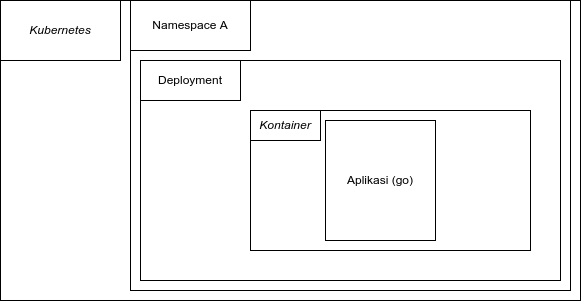
\includegraphics[width=0.6\textwidth]{pics/AplikasiDalamKubernetes.png}
	\caption{Kontainer berada di dalam \textit{environment} kubernetes}
	\label{fig:aplikasiDiDalamKubernetes}
\end{figure}

\subsection{Akses ke Aplikasi Pihak Ketiga}
Agar dapat berjalan dengan baik, aplikasi membutuhkan akses kepada \textit{database}, Vault Client, dan Amazon S3 Client milik GudangAda. Oleh karena itu perlu sambungan dari aplikasi ke masing masing klien. \textit{Credentials} untuk menghubungkan ke masing klien diberikan oleh \textit{serviceaccount} yang menempelkan \textit{credentials} tersebut ke \textit{environment} variabel pada kontainer aplikasi. Gambar \ref{fig:aplikasiMendapatCredentials} memperlihatkan kondisi aplikasi pada lingkungan Kubernetes setelah mendapat akses \textit{credentials} dan terhubung ke klien pihak ketiga.

\begin{figure}
	\centering
	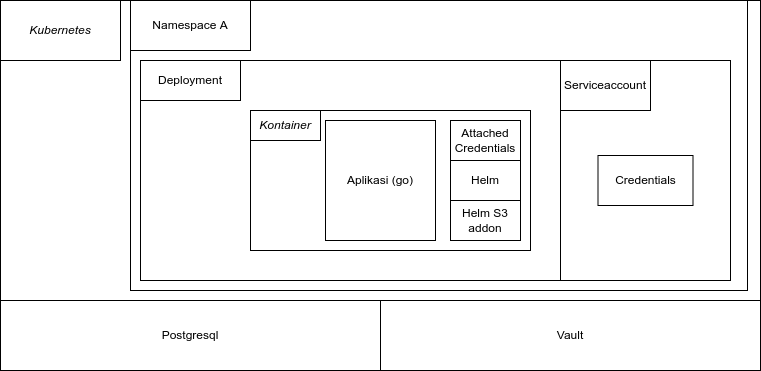
\includegraphics[width=0.75\textwidth]{pics/AplikasiMendapatCredentials.png}
	\caption{Aplikasi mendapat koneksi ke \textit{Database}, Vault \textit{client}, Amazon S3 \textit{Client}}
	\label{fig:aplikasiMendapatCredentials}
\end{figure}


\newpage

\subsection{Pengendalian \textit{Deployment} Pada Kubernetes}

Aplikasi perlu dapat mengendalikan banyak \textit{deployment} yang terdapat pada \textit{namespace} yang berbeda-beda. Oleh karena itu, \textit{serviceaccount} aplikasi perlu diberikan akses kepada \textit{namespace-namespace} yang akan dikendalikan.

\begin{figure}
	\centering
	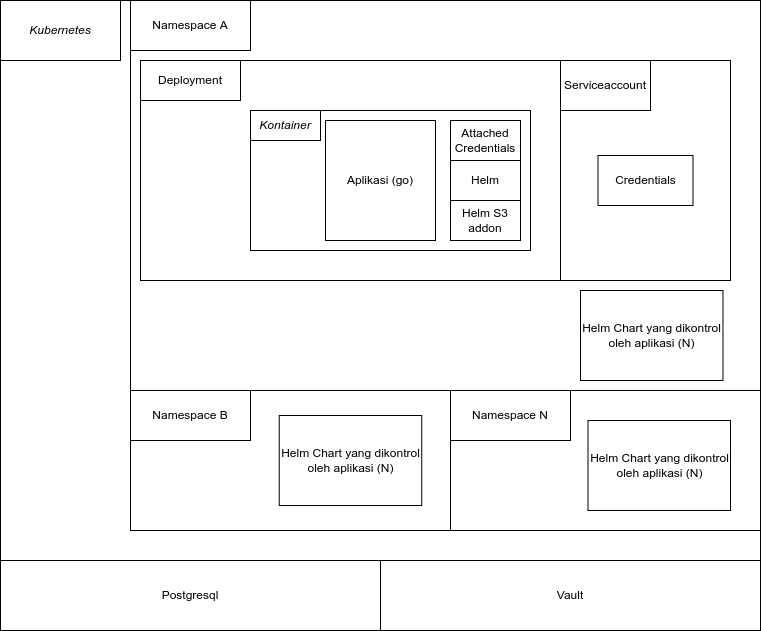
\includegraphics[width=0.85\textwidth]{pics/AplikasiMengontrolDeployment.png}
	\caption{Aplikasi mengontrol \textit{deployment}}
	\label{fig:aplikasiMengontrolDeployment}
\end{figure}

\newpage

\subsection{Akses Pengguna ke Aplikasi}

Agar dapat diakses oleh pengguna, perlu akses dari luar untuk dapat mengirimkan perintah ke aplikasi. Untuk memastikan orang yang dapat mengakses aplikasi merupakan orang yang berhak, dibutuhkan implementasi fitur otorisasi. Sayangnya, fitur otorisasi tidak termasuk ke dalam rancangan \textit{Minimum Viable Product}(MVP) aplikasi yang ditetapkan oleh perusahaan.

Sehingga pada penelitian kali ini, akses dari pengguna tidak dapat dilakukan dengan sambungan ke \textit{internet}. Akses ke aplikasi dilakukan dengan cara membuat \textit{port forward} dari \textit{Deployment} aplikasi ke perangkat pengguna setiap kali pengguna ingin mengakses aplikasi seperti gambar \ref{fig:arsitekturFinalAplikasi}. Pengguna yang ingin melakukan \textit{port forward} harus memiliki akses ke Kubernetes Cluster yang dikendalikan oleh aplikasi. Hal ini dilakukan untuk membatasi akses aplikasi ke pengguna yang berhak.


\begin{figure}
	\centering
	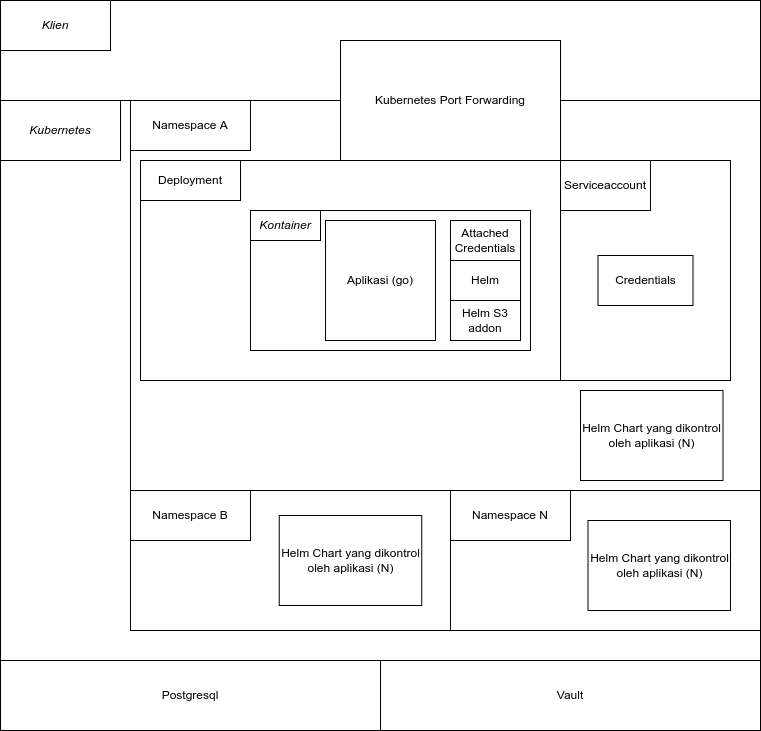
\includegraphics[width=1\textwidth]{pics/ArsitekturFinalAplikasi.png}
	\caption{Penggunaan aplikasi melalui \textit{port forwarding}}
	\label{fig:arsitekturFinalAplikasi}
\end{figure}



\section{Perancangan Arsitektur Aplikasi}
\label{sec:perancanganArsitektur}

Bagian ini menjelaskan mengenai desain aplikasi yang meliputi: justifikasi pemilihan teknologi, desain utama aplikasi, desain \textit{templating engine}, dan desain\textit{ secret engine}.

\subsection{Pemilihan Teknologi}
\label{sec:pemilihanTeknologi}
Penulis akan mengembangkan aplikasi menggunakan bahasa pemrograman Go. Pemilihan ini didasarkan karena hampir semua aplikasi pihak ketiga dikembangkan menggunakan Golang dan API disediakan dalam bentuk \textit{library} Go. Selain itu, sebagian besar \textit{Engineer} pada tim data GudangAda menggunakan bahasa pemrograman Go, sehingga mengembangkan aplikasi dengan menggunakan Go akan mempermudah pengembangan aplikasi ke depannya.

\subsection{Desain Utama Aplikasi}
\label{sec:desainUtamaAplikasi}
Aplikasi yang dikembangkan akan menggunakan arsitektur \textit{Controller-Service-Repository} dimana permintaan yang masuk akan diterima oleh \textit{router} yang kemudian akan diarahkan ke masing-masing \textit{controller} untuk diproses. Setelah masuk ke \textit{controller}, data dari permintaan akan di \textit{parse} untuk selanjutnya diarahkan ke \textit{services}. \textit{Services} akan menjalankan logika bisnis untuk mencatat dan verifikasi permintaan yang masuk. Setelah itu \textit{Sevices} akan memanggil \textit{repository} yang akan mengirimkan perintah \textit{deployment} kepada Helm API, \textit{database} dan/atau Amazon Kinesis API. Rancangan awal aplikasi dapat dilihat pada gambar \ref{fig:rancanganAwalAplikasi}.


\begin{figure}
	\centering
	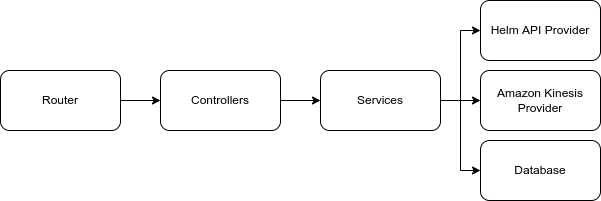
\includegraphics[width=1\textwidth]{pics/rancanganAplikasiAwal.png}
	\caption{Desain Aplikasi}
	\label{fig:rancanganAwalAplikasi}
\end{figure}

Di dalam \textit{service} terdapat \textit{templating engine} yang dapat melakukan \textit{parsing request} asli ke dalam spesifikasi akhir dan \textit{Vault engine} yang akan memasukkan variabel rahasia ke dalam aplikasi.

\subsection{\textit{Templating Engine}}
\label{sec:templatingEngine}
Untuk memenuhi kebutuhan K4, dibutuhkan sistem \textit{template} dimana pengguna dapat mendefinisikan sebuah \textit{template} pada aplikasi dan melakukan \textit{deployment} berdasarkan \textit{template} tersebut.\textit{ Templating engine} milik Golang akan digunakan untuk melakukan \textit{templating} pada aplikasi yang dikerjakan. 

\begin{figure}
	\centering
	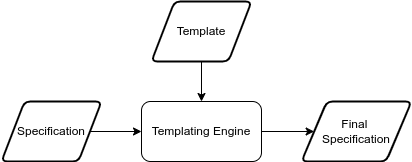
\includegraphics[width=0.7\textwidth]{pics/TemplatingEngine.png}
	\caption{Alur kerja \textit{templating engine}}
	\label{fig:alurTemplatingEngine}
\end{figure}

Pada gambar \ref{fig:alurSecretEngine} dapat dilihat bahwa dibutuhkan \textit{template} dan spesifikasi \textit{deployment} untuk mendapatkan spesifikasi akhir. Pengguna dapat membuat definisi \textit{template} yang akan ditambahkan kedalam \textit{database}. Setelah itu, pengguna dapat mengirimkan spesifikasi dari \textit{deployment} berdasarkan \textit{template} yang telah didefinisikan. Sebagai contoh, jika ada definisi \textit{template} \ref{code:templateFile} dan spesifikasi \textit{deployment} \ref{code:templateValue}, maka akan terbentuk \ref{code:finalTemplate} yang akan dikirimkan kepada Helm API untuk dibuatkan \textit{deployment}.

\begin{lstlisting}[frame=single,caption={Contoh file \textit{template}},label={code:templateFile}]
chart:
- release_name: {{ .Values.name }}
  name: {{ .Values.chart.name }}
  namespace: {{ .Values.namespace }}
  version: {{ .Values.chart.version }}
\end{lstlisting}

\begin{lstlisting}[frame=single,caption={Contoh nilai yang dipakai},label={code:templateValue}]
name: regular-deployment
namespace: default
chart:
    name: nginx
    version: 1.0.0
\end{lstlisting}

\begin{lstlisting}[frame=single,caption={Hasil akhir \textit{template}},label={code:finalTemplate}]
chart:
- release_name: regular-deployment
  name: nginx
  namespace: default
  version: 1.0.0
\end{lstlisting}

\subsection{Secret Engine}
\label{sec:vaultEngine}

Spesifikasi \textit{deployment} sering kali mengandung variabel rahasia yang sebaiknya tidak diketahui oleh banyak orang. Oleh karena itu, variabel tersebut disembunyikan pada Vault yang aman dan memiliki akses yang terbatas. Aplikasi membutuhkan cara agar dapat mendapatkan variabel tersebut tanpa diketahui nilainya oleh orang yang melakukan proses \textit{deployment}.

Untuk memenuhi kebutuhan di atas, dibutuhkan integrasi dengan Vault dimana aplikasi dapat mengakses variabel rahasia yang tersimpan tanpa campur tangan langsung dari pengguna. Pengguna hanya perlu memberikan alamat dari variabel rahasia dan aplikasi akan mengakses variabel tersebut. 

\begin{figure}
	\centering
	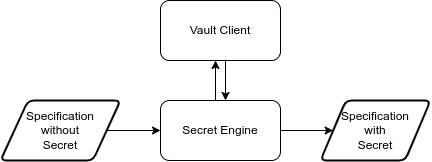
\includegraphics[width=0.7\textwidth]{pics/SecretEngine.png}
	\caption{Alur kerja \textit{secret engine}}
	\label{fig:alurSecretEngine}
\end{figure}

Alur kerja\textit{ secret engine} dapat dilihat pada gambar \ref{fig:alurSecretEngine}. Sebagai contoh, pengguna akan membuat \textit{template} terlebih dahulu seperti kode \ref{code:secretTemplate} dan pengguna akan memberikan alamat variabel pada Vault pada kode \ref{code:secretValue}, jika pada Vault terdapat \textit{key} 'kv/data/devops/regular-deployment' dan \textit{secret} 'DB-password' yang bernilai 'super-secret-password', maka aplikasi akan menggantikan nilai '.Values.secret.Vault.DBPass' menjadi 'super-secret-password' seperti kode \ref{code:secretFinal}.

\begin{lstlisting}[frame=single,caption={Contoh penggunaan \textit{secret} pada template},label={code:secretTemplate}]
name: regular-deployment
namespace: default
chart:
    name: nginx
    version: 1.0.0
    values:
        databasePassword: {{ .Values.secret.Vault.DBPass }}
\end{lstlisting}

\begin{lstlisting}[frame=single,caption={Contoh penggunaan \textit{secret} pada nilai yang dipakai},label={code:secretValue}]
secret:
  Vault:
    DBPass: kv/data/devops/regular-deployment:DB-password
\end{lstlisting}

\begin{lstlisting}[frame=single,caption={Contoh penggunaan \textit{secret} pada nilai yang dipakai},label={code:secretFinal}]
secret:
  Vault:
    DBPass: super-secret-password
\end{lstlisting}


